\documentclass[a4paper]{article}
%\usepackage{fixltx2e} % LaTeX patches, \textsubscript
%\usepackage{cmap} % fix search and cut-and-paste in Acrobat
\usepackage[T1]{fontenc}
\usepackage[utf8]{inputenc}
\usepackage{amsmath}
\usepackage{graphicx}
\usepackage{mathptmx} % Times
\usepackage[scaled=.90]{helvet}
\usepackage{courier}
\usepackage[margin=0.5in]{geometry}
\usepackage{xcolor}
\usepackage{longtable}
%%% User specified packages and stylesheets
\DeclareGraphicsExtensions{ %
    .pdf,.PDF,%
    .png,.PNG,%
    .jpg,.mps,.jpeg,.jbig2,.jb2,.JPG,.JPEG,.JBIG2,.JB2}
\title{PyRETIS --- analysis of MD flux results}
\author{}
\date{}

\begin{document}
\maketitle
\noindent Initial flux report generated by PyRETIS version 3.0.3
on 19.04.2026 12:15:29.
\\
\noindent The main results are the initial fluxes:

\begin{longtable}{| c | c | c | c | c | c | c | c | c |}
\caption{Flux for interfaces}\\
\hline
Int. & Position & Flux / units & Error & Rel. error & Ncross & Neffcross & Neffcross/Ncross & Steps per cross\\ \hline
 1   & -0.9000  & $ 0.000000 $ & $   nan    $ & $   nan    $ & $   0    $ & $   0    $ & $   nan    $ & $   inf    $\\
\hline
\end{longtable}

\noindent Detailed results are given below and
the flux results are summarized in the
section on MD flux data.

\section{Results from the MD flux analysis}
The following figures were generated by the
analysis program:

\subsection{MD energy data}
Energy and the running average of the energy:
\begin{center}
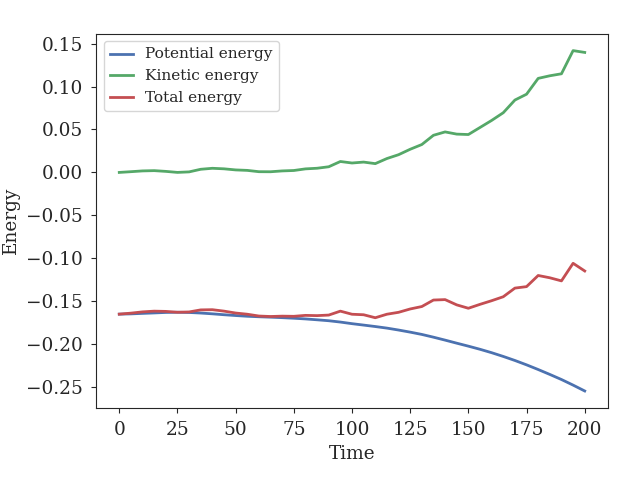
\includegraphics[width=0.45\linewidth]{energies.png}%
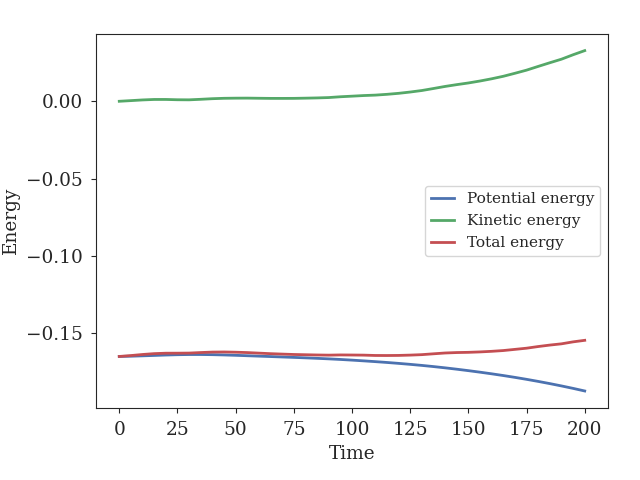
\includegraphics[width=0.45\linewidth]{runenergies.png}%
\end{center}
Temperature and running average of temperature:
\begin{center}
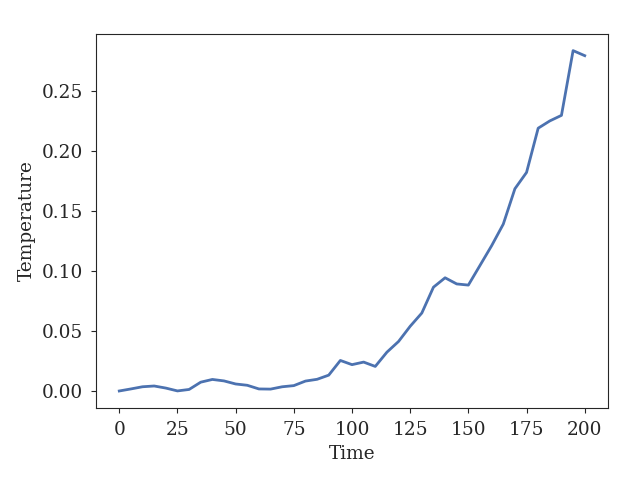
\includegraphics[width=0.45\linewidth]{temperature.png}%
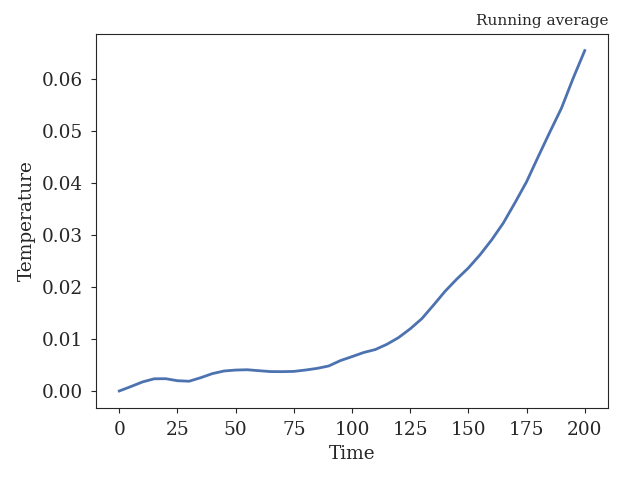
\includegraphics[width=0.45\linewidth]{runtemperature.png}%
\end{center}
Block error analysis:
\begin{center}
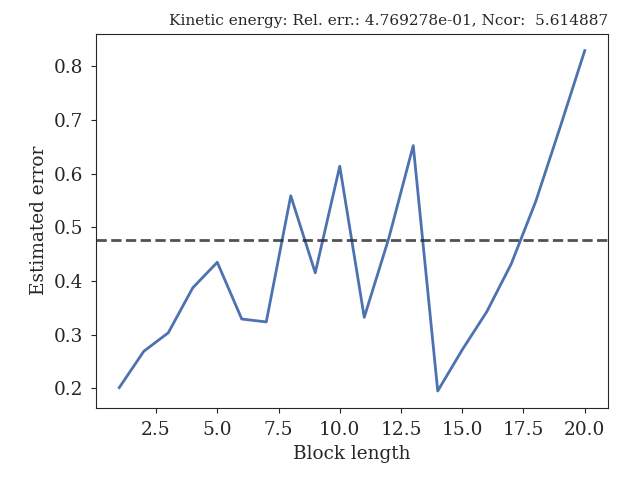
\includegraphics[width=0.30\linewidth]{ekinblock.png}%
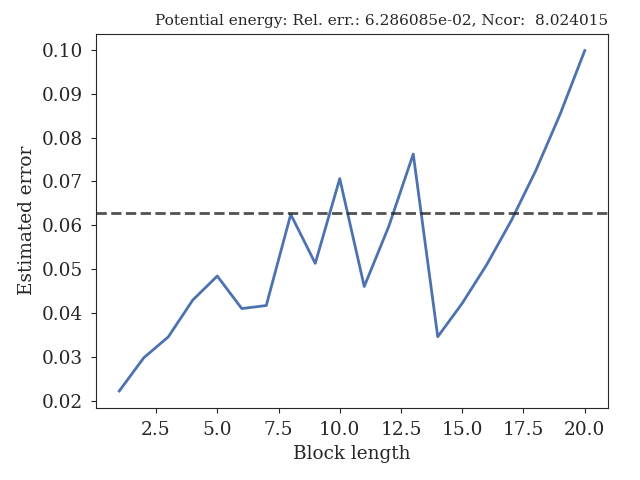
\includegraphics[width=0.30\linewidth]{vpotblock.png}%
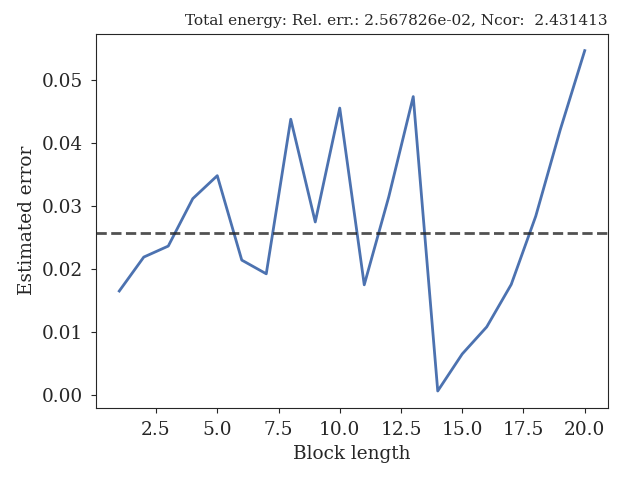
\includegraphics[width=0.30\linewidth]{etotblock.png}%
\end{center}
Distribution of energies:
\begin{center}
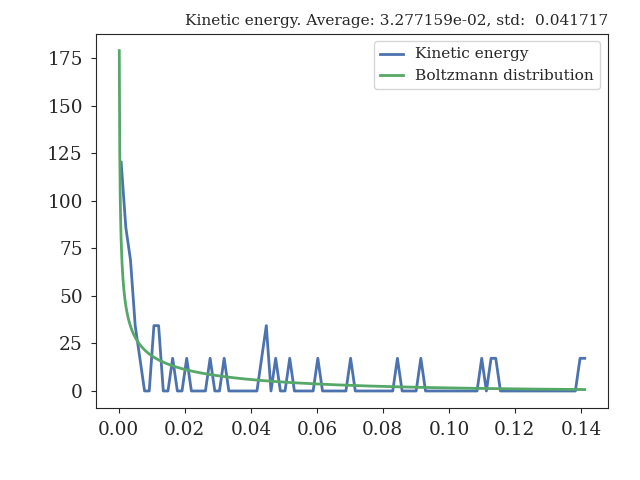
\includegraphics[width=0.30\linewidth]{ekindist.png}%
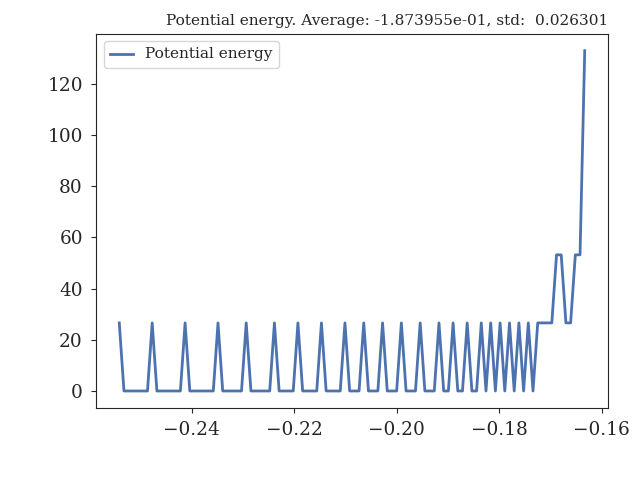
\includegraphics[width=0.30\linewidth]{vpotdist.png}%
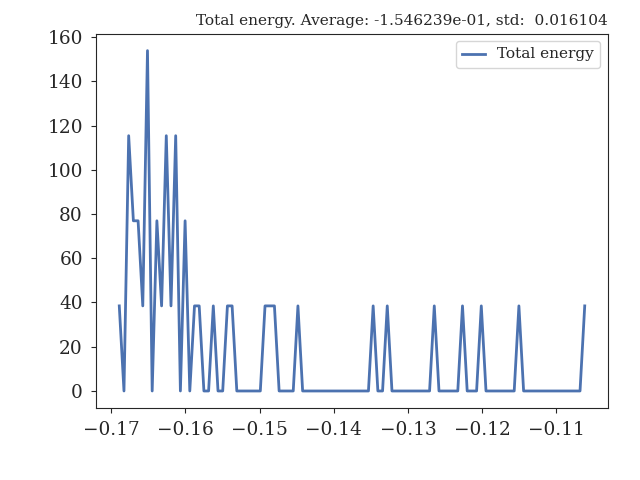
\includegraphics[width=0.30\linewidth]{etotdist.png}%
\end{center}
Block error and distribution of temperature:
\begin{center}
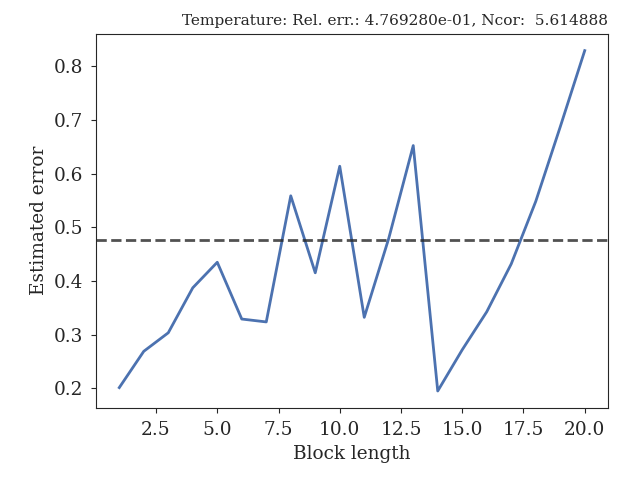
\includegraphics[width=0.30\linewidth]{tempblock.png}%
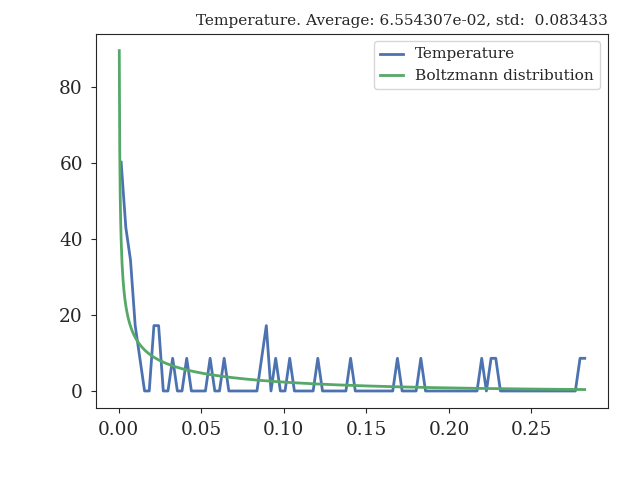
\includegraphics[width=0.30\linewidth]{tempdist.png}%
\end{center}

\subsection{MD order parameter data}
\begin{center}
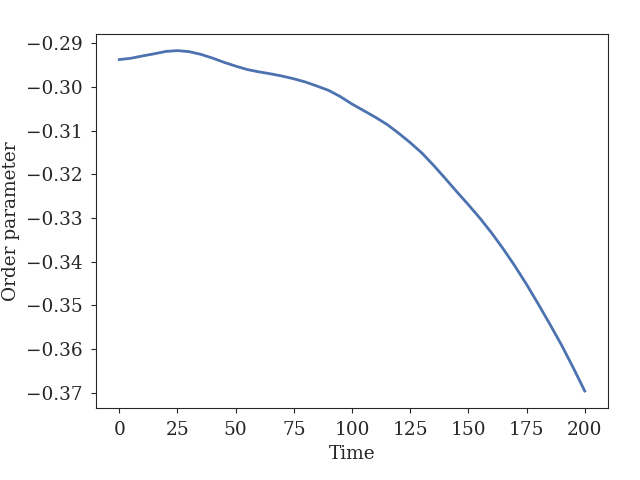
\includegraphics[width=0.30\linewidth]{order.png}%
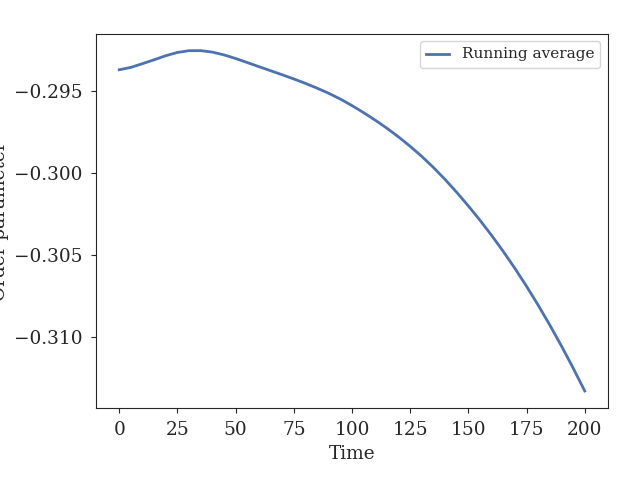
\includegraphics[width=0.30\linewidth]{runorder.png}%
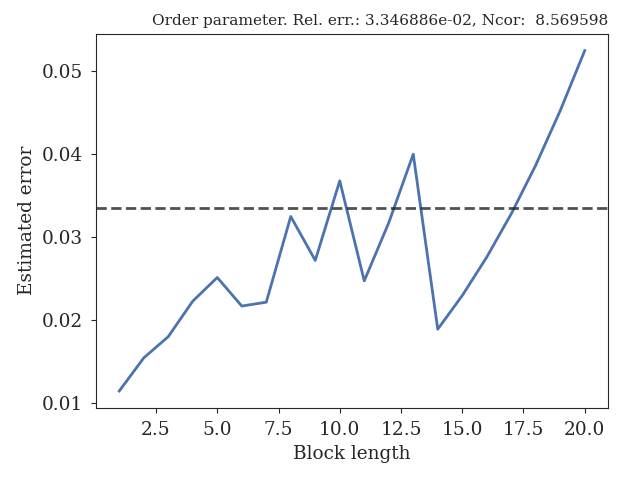
\includegraphics[width=0.30\linewidth]{ordererror.png}%
\end{center}
\begin{center}
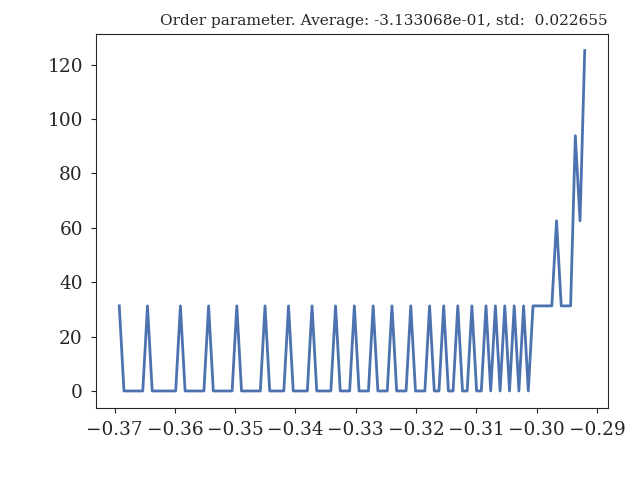
\includegraphics[width=0.30\linewidth]{orderdist.png}%
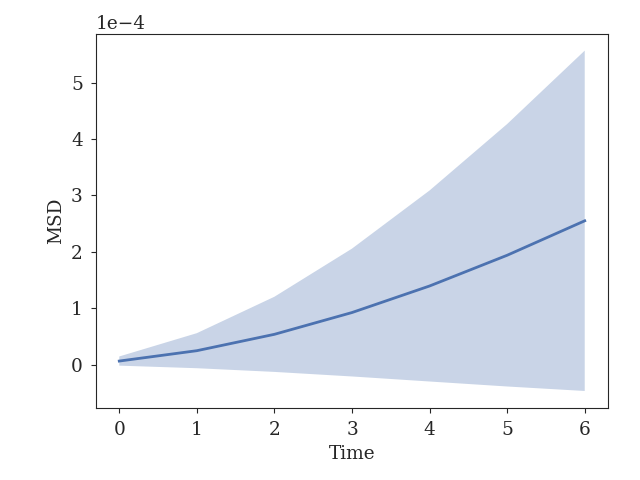
\includegraphics[width=0.30\linewidth]{ordermsd.png}%

\end{center}
\subsection{MD flux data}

\begin{center}
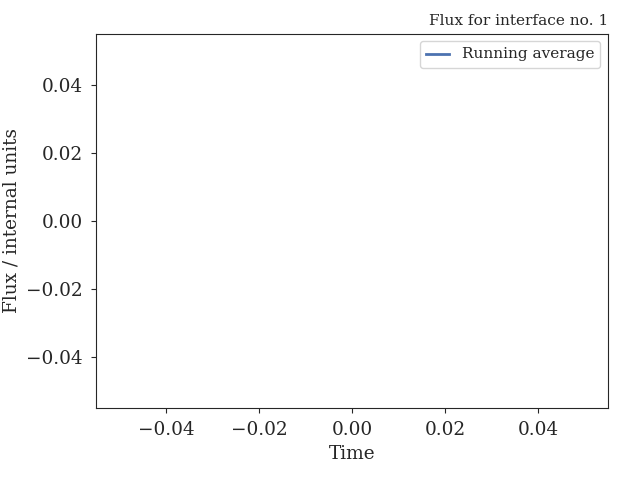
\includegraphics[width=0.45\linewidth]{runflux_1.png}%
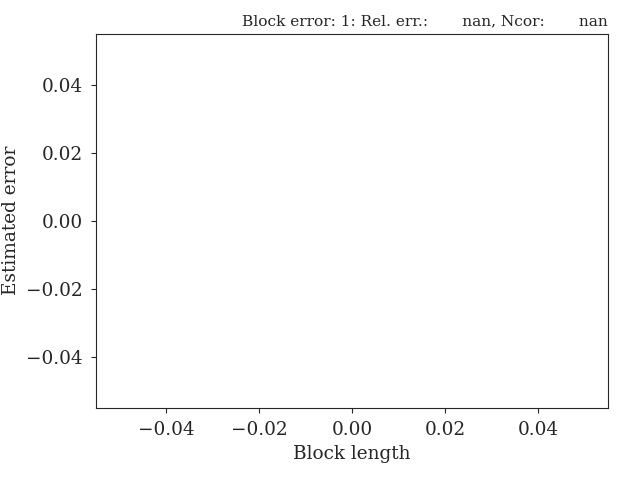
\includegraphics[width=0.45\linewidth]{errflux_1.png}%
\end{center}


\begin{longtable}{| c | c | c | c | c | c | c | c | c |}
\caption{Flux for interfaces}\\
\hline
Int. & Position & Flux / units & Error & Rel. error & Ncross & Neffcross & Neffcross/Ncross & Steps per cross\\ \hline
 1   & -0.9000  & $ 0.000000 $ & $   nan    $ & $   nan    $ & $   0    $ & $   0    $ & $   nan    $ & $   inf    $\\
\hline
\end{longtable}

\begin{longtable}{| c | c |}
\caption{Cycles spent in state}\\
\hline
State & Cycles\\ \hline
A &      200\\
B &        0\\
overall A &      200\\
overall B &        0\\
Total cycles &      200\\
\hline
\end{longtable}

\begin{longtable}{| c | c | c | c | c |}
\caption{Efficiency}\\
\hline
Interface & $p_\text{MD}$ & $\frac{1-p}{p}$ & Efficiency time & Correlation\\ \hline
    1      & $ 0.000000 $ & $   inf    $ & $   nan    $ & $   nan    $\\
\hline
\end{longtable}
\end{document}